\documentclass{InsightArticle}

\usepackage[dvips]{graphicx}
\usepackage{float}
\usepackage{subfigure}

\usepackage[dvips,
bookmarks,
bookmarksopen,
backref,
colorlinks,linkcolor={blue},citecolor={blue},urlcolor={blue},
]{hyperref}

\title{Closed Loop Simplification}

% 
% NOTE: This is the last number of the "handle" URL that 
% The Insight Journal assigns to your paper as part of the
% submission process. Please replace the number "1338" with
% the actual handle number that you get assigned.
%
\newcommand{\IJhandlerIDnumber}{3250}

% Increment the release number whenever significant changes are made.
% The author and/or editor can define 'significant' however they like.
\release{0.00}

% At minimum, give your name and an email address.  You can include a
% snail-mail address if you like.

\author{David Doria}
\authoraddress{Army Research Laboratory, Aberdeen MD}


\begin{document}

\IJhandlefooter{\IJhandlerIDnumber}


\ifpdf
\else
   %
   % Commands for including Graphics when using latex
   % 
   \DeclareGraphicsExtensions{.eps,.jpg,.gif,.tiff,.bmp,.png}
   \DeclareGraphicsRule{.jpg}{eps}{.jpg.bb}{`convert #1 eps:-}
   \DeclareGraphicsRule{.gif}{eps}{.gif.bb}{`convert #1 eps:-}
   \DeclareGraphicsRule{.tiff}{eps}{.tiff.bb}{`convert #1 eps:-}
   \DeclareGraphicsRule{.bmp}{eps}{.bmp.bb}{`convert #1 eps:-}
   \DeclareGraphicsRule{.png}{eps}{.png.bb}{`convert #1 eps:-}
\fi


\maketitle


\ifhtml
\chapter*{Front Matter\label{front}}
\fi

\begin{abstract}
\noindent

This document presents an implementation of an algorithm to find a low edge-count approximation of a complex, discrete, 2D closed contour. This implementation is based on the algorithm described in ``Using Aerial Lidar Data to Segment And Model Buildings'' and ``A Bayesian Approach to Building Footprint Extraction from Aerial LIDAR Data.''

The code is available here:
https://github.com/daviddoria/ClosedLoopSimplification

\end{abstract}

\IJhandlenote{\IJhandlerIDnumber}

\tableofcontents
%%%%%%%%%%%%%%%%%%%%
\section{Introduction}
This document presents an implementation of an algorithm to find a low edge-count approximation of a complex, discrete, 2D closed contour. Our goal is to represent the outline of an object in a simple fashion. This type of algorithm is commonly found in applications involving building detection from aerial LiDAR data.

This implementation is based on the algorithm described in \cite{WangThesis} and \cite{WangPaper}.

%%%%%%%%%%%%%%%%%%%%
\section{Algorithm}
\label{sec:Algorithm}
\subsection{Input}
\label{sec:Algorithm:Input}
The input to this algorithm is an ordered set of points describing a closed loop. In Figure \ref{fig:Input} we show a synthetic example of such a data set.

\begin{figure}[H]
  \centering
  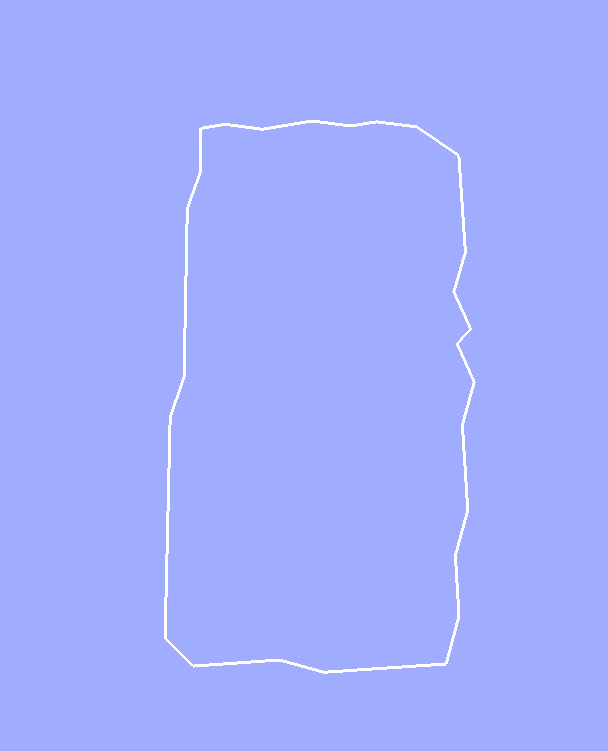
\includegraphics[width=0.3\linewidth]{images/input}
  \caption{A closed 2D contour.}
  \label{fig:Input}
\end{figure}

%%%%%%%%%%%%%%%%%%%%
\subsection{Contour Simplification}
\label{sec:Algorithm:ContourSimplification}
It is often desirable to reduce a contour to a simpler approximation of the same shape. For example, in the case of building detection, we often want to represent a building as a rectangle (4 line segments). Depending on the density of the input, the boundary at this point could be represented by hundreds of line segments, mostly describing the noise in the data. To reduce the number of line segments in the boundary, we use the following procedure:
\begin{itemize}
 \item Create a directed graph of the contour using exactly the vertices of the rough boundary as the vertices and the ordered line segments of the rough boundary as directed edges.
 \item Attempt to add every other possible edge (from each vertex to every other vertex ahead of it in the contour ordering) only if the new edge passes a straightness test.
 \item The straightness test is described in \cite{WangThesis} as the sum of the distances from every point between the two end points to the proposed edge. We have found it more convenient to set this threshold based on the average of these distances, as the length of the edges then is not a factor in determining the straightness criteria.
\begin{figure}[H]
  \centering
  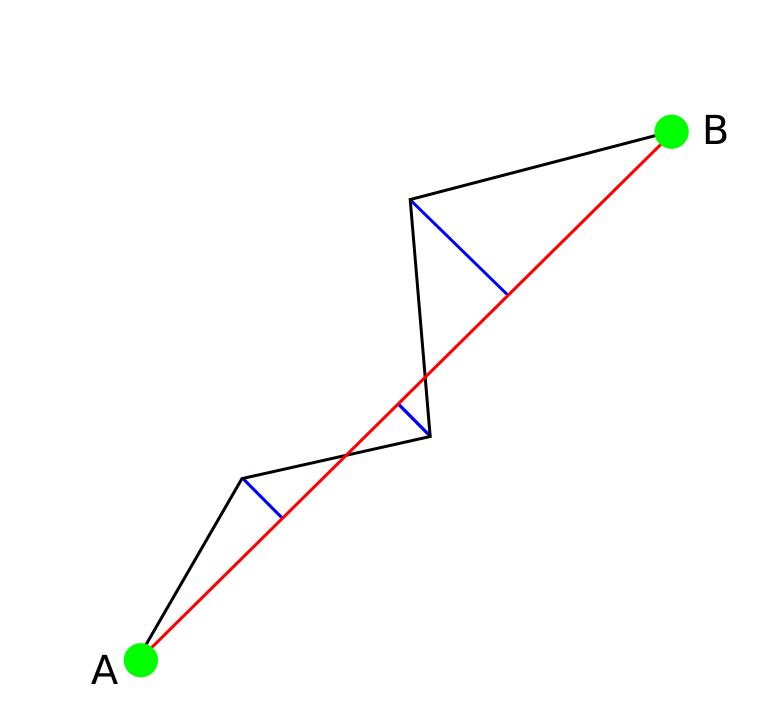
\includegraphics[width=0.3\linewidth]{images/straightness}
  \caption{The straightness computation of a proposed edge between vertices A and B. Black: the rough boundary. Red: the proposed edge. Blue: the distances from all points on the boundary between A and B to the proposed edge.}
  \label{fig:Straightness}
\end{figure}
 \item By finding any full loop shortest path on this graph, we will have significantly improved (i.e. reduced the line count of) our boundary. However, it is not a well posed graph theoretic problem to ask for the shortest path from a vertex to itself (a loop) and expect a non-zero answer (i.e. the shortest path from a vertex to itself is to not move at all!). To remedy this, we add the ordered vertices around the boundary twice, as well as duplicate the edges on this second loop of vertices. Now we can ask for the shortest path from vertex $i$ to vertex $i+N$ where $N$ is the original number of vertices in the rough boundary.
 \item If we compute this shortest path from any random vertex, we will have a solution to our original problem of finding a low-line segment count approximation to the boundary. However, the choice of starting vertex actually can change the solution, though often only slightly. Because of this, we find the shortest path starting at all vertices, and choose the shorest one as our solution.
\end{itemize}

[Demonstrate the case where the starting point is not on the best shortest path. This is why we must find all shortest paths from all points, not just one.]

%%%%%%%%%%%%%%%%%%%%
\section{Demonstration}
\label{sec:Demonstration}

% \begin{figure}[H]
% \centering
% \subfigure[Image to be filled. The region to be filled is shown in bright green.]
%   {
%   \includegraphics[width=0.3\linewidth]{images/BlackWhite}
%   \label{fig:SyntheticDemonstration:ExampleInputImage}
%   }
% \subfigure[The mask of the region to inpaint.]
%   {
%   \includegraphics[width=0.3\linewidth]{images/BlackWhiteMask}
%   \label{fig:SyntheticDemonstration:ExampleInputMask}
%   }
% \subfigure[The result of the inpainting.]
%   {
%   \includegraphics[width=0.3\linewidth]{images/BlackWhiteResult}
%   \label{fig:SyntheticDemonstration:ExampleInputOutput}
%   }
% \caption{Synthetic Demonstration}
% \label{fig:SyntheticDemonstration}
% \end{figure}

%%%%%%%%%%%%%%%
\section{Code Snippet}

\begin{verbatim}

\end{verbatim}

%%%%%%%%%%%
\section{Future Work}
In the polygonal approximation, there is a minimum straightness parameter which must be set which has a major impact on the resulting simplification. Removing the need to manually specify this parameters would make this algorithm more robust to different data types, as well as provide the best possible results on any particular data set.

%%%%%%%%%%%%%%%
\begin{thebibliography}{9}

	\bibitem{WangThesis}
	  Wang, O.,
	  \emph{Using Aerial Lidar Data to Segment And Model Buildings}.
	  University Of California Santa Cruz Masters Thesis, 2006


	\bibitem{WangPaper}
	  Wang. O, Lodha. S, Helmbold, D.,
	  \emph{A Bayesian Approach to Building Footprint Extraction from Aerial LIDAR Data}.
	  3D Data Processing, Visualization, and Transmission 2006

\end{thebibliography}

\end{document}